\documentclass[11pt, addpoints, answers]{exam}

\usepackage{amsmath, amssymb, euler}
\usepackage{xcolor}
\usepackage{algorithm, algorithmicx, algpseudocode}
\usepackage{tikz, tikz-qtree, drawstack}
\usepackage[shortlabels]{enumitem}

\usetikzlibrary{graphs}
\tikzset{every tree node/.style={minimum width=2em,draw,circle},
	blank/.style={draw=none},
	edge from parent/.style=
	{draw,edge from parent path={(\tikzparentnode) -- (\tikzchildnode)}},
	level distance=1.2cm}

% For inserting code snippets.
\usepackage{listings}
\lstset{
    columns = fixed,
    basewidth = {0.5em},
    breaklines = true,
    backgroundcolor = \color{white},
    keywordstyle = \color[RGB]{40, 40, 255},
    numberstyle = \footnotesize\color{darkgray},
    commentstyle = \ttfamily\color{violet},
    basicstyle = \ttfamily,
    stringstyle = \ttfamily\color[RGB]{128, 0, 0},
    showstringspaces = false,
    language = {[11]C++},
    escapechar = \@
}
\lstnewenvironment{cpp}[1][]{\lstset{language = {[11]C++}, #1}}{}

\usepackage{tikz}

% headers, footers, titles
\newcommand{\CourseName}{CS101 Algorithms and Data Structures}
\newcommand{\HomeworkNO}{Homework 9}
\newcommand{\DueDate}{Due date: 23:59, November 27th, 2022}

\pagestyle{headandfoot}
\runningheadrule
\runningheader{\CourseName}{\HomeworkNO}{\DueDate}
\runningfooter{}{\thepage}{}

\title{
	\CourseName\\
	Fall 2022\\
	\HomeworkNO
}
\author{}
\date{\DueDate}

% formats of questions, choices, points, etc.
\qformat{\bf\thequestion. (\totalpoints\ points) \thequestiontitle\hfill}
\pointname{'}
\CorrectChoiceEmphasis{\bf\color{blue}}

% We frequently use this font.
\newcommand{\ttt}{\texttt}
\newcommand{\blue}[1]{\textcolor{blue}{#1}}
\newcommand{\bluett}[1]{\blue{\ttt{#1}}}

\begin{document}

\maketitle

\begin{enumerate}
	\item Please write your solutions in English.
	\item Submit your solutions to gradescope.com.
	\item Set your FULL name to your Chinese name and your STUDENT ID correctly in Account Settings.
	\item If you want to submit a handwritten version, scan it clearly. \ttt{CamScanner} is recommended.
	\item When submitting, match your solutions to the problems correctly.
	\item No late submission will be accepted.
	\item Violations to any of the above may result in zero points.
\end{enumerate}

\newpage

\begin{questions}

\titledquestion{Multiple Choices}

Each question has \textbf{one or more than one} correct answer(s). Please answer the following questions \textbf{according to  the definition specified in the lecture slides}.

%%%%%%%%%%%%%%%%%%%%%%%%%%%%%%%%%%%%%%%%%%%%%%%%%%%%%%%%%%%%%%%%%%%%%%%%%%%
% Note: The `LaTeX' way to answer a multiple-choices question is to replace `\choice'
% with `\CorrectChoice', as what you did in the previous questions. However, there are 
% still many students who would like to handwrite their homework. To make TA's work 
% easier, you have to fill your selected choices in the table below, no matter whether 
% you use LaTeX or not.
%%%%%%%%%%%%%%%%%%%%%%%%%%%%%%%%%%%%%%%%%%%%%%%%%%%%%%%%%%%%%%%%%%%%%%%%%%%

\begin{table}[htbp]
	\centering
	\begin{tabular}{|p{2cm}|p{2cm}|p{2cm}|p{2cm}|}
		\hline
		(a) & (b) & (c) & (d)\\
		\hline
		%%%%%%%%%%%%%%%%%%%%%%%%%%%%%%%%%%%%%%%%%%%%%%%%%%%%%%%%%%
		% YOUR ANSWER HERE.
		 ACD   & AC    &  ABD   & ABCD\\
		%%%%%%%%%%%%%%%%%%%%%%%%%%%%%%%%%%%%%%%%%%%%%%%%%%%%%%%%%%
		\hline
	\end{tabular}
\end{table}

\begin{parts}
	\part[3] Which of the following statements about \textbf{topological sort} is/are true?

	\begin{choices}
        \CorrectChoice Implementation of topological sort requires $O(|V|)$ extra space.
        \choice Since we have to scan all vertices to find those with zero in-degree in each iteration, the run time of topological sort is $\Omega(|V|^2)$.
        \CorrectChoice Any sub-graph of a DAG has a topological sorting.
        \CorrectChoice Any directed tree has a topological sorting.
	\end{choices}

	\part[3] Which of the following statements about \textbf{Dijkstra’s algorithm} is/are true?

	\begin{choices}
        \CorrectChoice If we implement Dijkstra’s algorithm with a binary min-heap, we may change keys of internal nodes in the heap.
        \choice Dijkstra’s algorithm can find the shortest path in any DAG.
        \CorrectChoice If we use Dijkstra’s algorithm, whether the graph is directed or undirected does not matter.
        \choice We prefer Dijkstra’s algorithm with binary heap implementation to the naive adjacency matrix implementation in a dense graph where $|E| = \Theta(|V|^2)$.
	\end{choices}

    \part[3] Which of the following statements about \textbf{Dijkstra’s algorithm} is/are true?

    \begin{choices}
        \CorrectChoice Dijkstra's algorithm with a binary heap could run in time $O((|V|+|E|) \log |V|)$.
        \CorrectChoice Dijkstra's algorithm with a Fibonacci heap could run in time $O(|E| + |V|\log |V|)$.
        \choice Dijkstra's algorithm on a tree with a binary heap could run in time $O(|E|+|V|)$.
        \CorrectChoice Dijkstra's algorithm with an adjacency list could run in time $O(|V|^2 + |E|)$.
    \end{choices}

	\part[3] Which of the following statements about \textbf{Bellman-Ford's algorithm} is/are true?
		
	\begin{choices}
        \CorrectChoice Topological sort can be extended to determine whether a graph has a cycle while Bellman-Ford's algorithm can be extended to determine whether a graph has a negative cycle.
        \CorrectChoice Bellman-Ford's algorithm can find the shortest path for negative-weighted directed graphs without negative cycles while Dijkstra’s algorithm may fail.
        \CorrectChoice Topological sort can find the critical path in a DAG while Bellman-Ford's algorithm can find the single-source shortest path in a DAG.
        \CorrectChoice The run time of Bellman-Ford's algorithm is $O(|V||E|)$, which is more time-consuming than Dijkstra’s algorithm with heap implementation.
	\end{choices}
\end{parts}

\newpage

\titledquestion{Topological Sort}

    Given the following DAG, run topological sort with a queue. Write down the vertex you select and update the in-degree \texttt{ind[i]} of all vertices in each iteration.  
	
	\textit{Note: When pushing several vertices into the queue at the same time, push them alphabetically. You are NOT required to show your queue at each step.}
	
	\vspace{1cm}

	\begin{figure}[htbp]
		\centering
		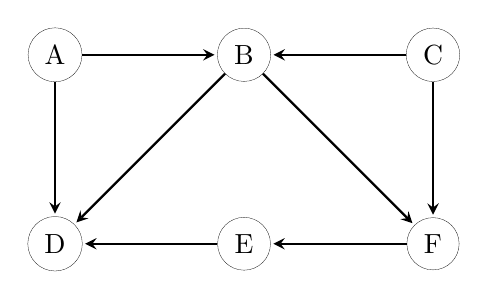
\begin{tikzpicture}[
			> = stealth, % arrow head style
			shorten > = 1pt, % don't touch arrow head to node
			node distance = 1cm, % distance between nodes
			thick, % line style
			scale = 0.8,
		]
		\node[circle, draw, line width=0.1pt] (a) at (-3,3){A};
		\node[circle, draw, line width=0.1pt] (b) at (0, 3){B};
		\node[circle, draw, line width=0.1pt] (c) at (3, 3){C};
		\node[circle, draw, line width=0.1pt] (d) at (-3,0){D};
		\node[circle, draw, line width=0.1pt] (e) at (0, 0){E};
		\node[circle, draw, line width=0.1pt] (f) at (3, 0){F};
		\draw[->] (a) to (b);
		\draw[->] (a) to (d);
		\draw[->] (b) to (d);
		\draw[->] (b) to (f);
		\draw[->] (c) to (b);
		\draw[->] (c) to (f);
		\draw[->] (f) to (e);
		\draw[->] (e) to (d);
		\end{tikzpicture}
	\end{figure}
	\vspace{0.5cm}

	\begin{table}[htbp]
		\begin{center}  
			\begin{tabular}{|l|c|l|l|l|l|l|l|}  
				\hline  
				 & vertex & \texttt{ind[A]} & \texttt{ind[B]} & \texttt{ind[C]} & \texttt{ind[D]} & \texttt{ind[E]} & \texttt{ind[F]}\\ \hline  
				initial     & / & 0  & 2  & 0  & 3  &  1 & 2  \\ \hline    
				iteration 1 & A  & 0  & 1  & 0  & 2  & 1  & 2  \\ \hline    
				iteration 2 & C  & 0  & 0  & 0  & 2  & 1  & 1  \\ \hline    
				iteration 3 & B  & 0  & 0  & 0  & 1  & 1  & 0  \\ \hline    
				iteration 4 & F  & 0  & 0  & 0  & 1  & 0  & 0  \\ \hline   
				iteration 5 & E  & 0  & 0  & 0  & 0  & 0  & 0  \\ \hline    
				iteration 6 & D  & 0  & 0  & 0  & 0  & 0  & 0  \\ 
				\hline  
			\end{tabular}  
		\end{center}
	\end{table}
	\vspace{0.5cm}



\begin{parts}
    \part[5] I. Fill in the table above. II. What is the topological sorting that you obtain?
    \begin{solution}
        %%%%%%%%%%%%%%%%%%%%%%%%%%%%%%%%%%%%%%%%%%%%%%%%%
        % Replace `\vspace{2in}' with your answer.
        %\vspace{1in}
        \\$A,C,B,F,E,D$
		%%%%%%%%%%%%%%%%%%%%%%%%%%%%%%%%%%%%%%%%%%%%%%%%%
    \end{solution}
    \part[3] How many different topological sortings does this graph have? Write them down.
    \begin{solution}
        %%%%%%%%%%%%%%%%%%%%%%%%%%%%%%%%%%%%%%%%%%%%%%%%%
        % Replace `\vspace{2in}' with your answer.
        %\vspace{1in}
        \\2
		\\$A,C,B,F,E,D$
		\\$C,A,B,F,E,D$
		%%%%%%%%%%%%%%%%%%%%%%%%%%%%%%%%%%%%%%%%%%%%%%%%%
    \end{solution}
\end{parts}

\newpage

\titledquestion{Dijkstra}[8]
Given the following weighted graph, run Dijkstra's algorithm by considering $A$ as the source vertex. Write down the vertex you select and update the distance \texttt{dis[i]} of all vertices in each iteration.

\begin{figure}[htbp]
    \centering
    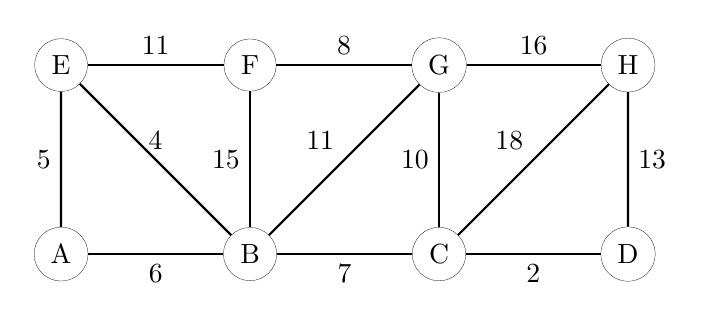
\begin{tikzpicture}
    [thick,scale=0.8, every node/.style={scale=1}]
    %		\node[circle] (n0){A};
    \node[circle, draw, line width=0.1pt] (a) at (-4.5,0){A};
    \node[circle, draw, line width=0.1pt] (b) at (-1.5,0){B};
    \node[circle, draw, line width=0.1pt] (c) at (1.5,0){C};
    \node[circle, draw, line width=0.1pt] (d) at (4.5,0){D};
    \node[circle, draw, line width=0.1pt] (e) at (-4.5,3){E};
    \node[circle, draw, line width=0.1pt] (f) at (-1.5,3){F};
    \node[circle, draw, line width=0.1pt] (g) at (1.5,3){G};
    \node[circle, draw, line width=0.1pt] (h) at (4.5,3){H};
    \draw[-] (a) to node[below]{6} (b);
    \draw[-] (a) to node[left]{5} (e);
    \draw[-] (b) to node[below]{7} (c);
    \draw[-] (b) to node[above]{4} (e);
    \draw[-] (b) to node[left]{15} (f);
    \draw[-] (b) to node[above left]{11} (g);
    \draw[-] (c) to node[below]{2} (d);
    \draw[-] (c) to node[left]{10} (g);
    \draw[-] (c) to node[above left]{18} (h);
    \draw[-] (d) to node[right]{13} (h);
    \draw[-] (e) to node[above]{11} (f);
    \draw[-] (f) to node[above]{8} (g);
    \draw[-] (g) to node[above]{16} (h);
    \end{tikzpicture}
\end{figure}
\vspace{0.5cm}


Fill in the table below.
\begin{table}[htbp]
    \begin{center}  
        \begin{tabular}{|l|c|c|c|c|c|c|c|c|c| p{3cm}|}  
            \hline  
            & vertex & \texttt{dis[A]} & \texttt{dis[B]} & \texttt{dis[C]} & \texttt{dis[D]} & \texttt{dis[E]} & \texttt{dis[F]} & \texttt{dis[G]} & \texttt{dis[H]}\\ \hline  
            initial 	& / & 0 &$\infty$&$\infty$&$\infty$&$\infty$&$\infty$&$\infty$&$\infty$\\ \hline
            iteration 1 & A  & 0  & 6  & $\infty$  & $\infty$  & 5  & $\infty$  &  $\infty$ & $\infty$ \\ \hline    
            iteration 2 & E  & 0  & 6  & $\infty$  & $\infty$  & 5  & 16  & $\infty$  & $\infty$ \\ \hline    
            iteration 3 & B  & 0  & 6  & 13  & $\infty$  & 5  & 16  &  17 & $\infty$ \\ \hline    
            iteration 4 & C  & 0  & 6  & 13  & 15  & 5  & 16  & 17 & 31 \\ \hline    
            iteration 5 & D  & 0  & 6  & 13  & 15  & 5  & 16  & 17  & 28 \\ \hline   
            iteration 6 & F  & 0  & 6  & 13  & 15  & 5  & 16  & 17  & 28 \\ \hline    
            iteration 7 & G  & 0  & 6  & 13  & 15  & 5  & 16  & 17  & 28 \\ \hline   
            iteration 8 & H  & 0  & 6  & 13  & 15  & 5  & 16  & 17  & 28 \\  
            \hline  
        \end{tabular}  
    \end{center}  
\end{table}


\newpage


\titledquestion{Providing Counterexamples}
For each of the following statements, provide counterexamples by \textbf{drawing a graph and briefly explaining it} to illustrate that these three statements are incorrect.

\begin{parts}
    \part[3] Each DAG with $|V|$ vertices and $|V|-1$ edges has its unique topological sorting.
    \begin{solution}
        %\vspace{3.5cm}
        \\
        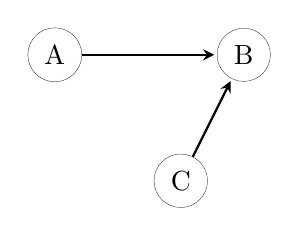
\begin{tikzpicture}[
            > = stealth, % arrow head style
            shorten > = 1pt, % don't touch arrow head to node
            node distance = 1cm, % distance between nodes
            thick, % line style
            scale = 0.8,
        ]
        \node[circle, draw, line width=0.1pt] (a) at (-3,3){A};
        \node[circle, draw, line width=0.1pt] (b) at (0, 3){B};
        \node[circle, draw, line width=0.1pt] (c) at (-1,1){C};
        \draw[->] (a) to (b);
        \draw[->] (c) to (b);
        \end{tikzpicture}
        \\
        it has two topological sorting results:\\
        $A,C,B$\\
        $C,A,B$
    \end{solution}
    \part[3] Since we can find a \textbf{maximum spanning tree} in a graph by multiplying all edge weights by $-1$ and then running Prim's algorithm, similarly we can find the \textbf{longest path} in a positive-weighted graph by negating all weights and running Dijkstra's algorithm from every source node.
    \begin{solution}
        % \vspace{4cm}
        \\\\
        \begin{tikzpicture}[
            > = stealth, % arrow head style
            shorten > = 1pt, % don't touch arrow head to node
            node distance = 1cm, % distance between nodes
            thick, % line style
            scale = 0.8,
        ]
        \node[circle, draw, line width=0.1pt] (a) at (-3,2){A};
        \node[circle, draw, line width=0.1pt] (b) at (0, 2){B};
        \node[circle, draw, line width=0.1pt] (c) at (-1.5,-0.5){C};
        \draw[->] (a) to node[up]{2} (b);
        \draw[->] (a) to node[left]{1} (c);
        \draw[->] (c) to node[right]{3} (b);
        \end{tikzpicture}
        \\
        if we set the source node be $A$, the terminal node be $B$, then after nagating all weights, the graph become\\\\
        \begin{tikzpicture}[
            > = stealth, % arrow head style
            shorten > = 1pt, % don't touch arrow head to node
            node distance = 1cm, % distance between nodes
            thick, % line style
            scale = 0.8,
        ]
        \node[circle, draw, line width=0.1pt] (a) at (-3,2){A};
        \node[circle, draw, line width=0.1pt] (b) at (0, 2){B};
        \node[circle, draw, line width=0.1pt] (c) at (-1.5,-0.5){C};
        \draw[->] (a) to node[up]{-2} (b);
        \draw[->] (a) to node[left]{-1} (c);
        \draw[->] (c) to node[right]{-3} (b);
        \end{tikzpicture}
        \\And when running Dijkstra's algorithm on the new graph from source node $A$, end at terminal node $B$.\\
        after the first time, node $B$ has the weight $-2$, which is less than $C$'s $-1$, so we will mark node $B$ as visited,
        and the final weight from $A$ to $B$ become $-2$, however, the shortest path on the new graph from $A$ to $B$ should be $-4$.
        so it is incorrect.\\
        $i.e.$ after negating all weights and running Dijkstra’s algorithm, we get the longest path $2$, however, it should be $4$.


    \end{solution}
    \newpage
    \part[3] Assume that we implement Dijkstra’s algorithm with a binary heap as the priority queue in a positive-weighted graph, then we can do the following operation: when the terminal vertex is pushed into the priority queue, we can stop the algorithm and return the correct shortest path from the source vertex to the terminal vertex, instead of keeping running the algorithm until popping the terminal vertex from the heap.
    \begin{solution}
        % \vspace{4cm}
        \\\\
        \begin{tikzpicture}[
            > = stealth, % arrow head style
            shorten > = 1pt, % don't touch arrow head to node
            node distance = 1cm, % distance between nodes
            thick, % line style
            scale = 0.8,
        ]
        \node[circle, draw, line width=0.1pt] (a) at (-3,2){A};
        \node[circle, draw, line width=0.1pt] (b) at (0, 2){B};
        \node[circle, draw, line width=0.1pt] (c) at (-1.5,-0.5){C};
        \draw[->] (a) to node[up]{10} (b);
        \draw[->] (a) to node[left]{1} (c);
        \draw[->] (c) to node[right]{1} (b);
        \end{tikzpicture}
        \\
        if we set the source node be $A$, the terminal node be $B$, then\\
        if stop the algorithm when pushed the terminal node into the priority queue, then the result is :\\
        the path is $A\to B$, and the total weight is $10$.\\
        but if stop the algorithm when popping the terminal node into the priority queue, then the result is :\\
        the path is $A\to C\to B$, and the total weight is $2$. which is better than the previous one.\\
        

    \end{solution}
\end{parts}


\end{questions}

\end{document}